%==============================================================================
\documentclass[11pt,oneside,onecolumn,letterpaper]{article}
\usepackage{times}
\usepackage[paperwidth=8.5in, paperheight=11in,
top=2.5cm, bottom=2.6cm, left=2.58cm, right=2.53cm]{geometry}
%\setlength{\textheight} {9.00in}
%\setlength{\textwidth}  {6.40in}
%\setlength{\topmargin}  {-0.50in}
%%\setlength{\headheight} {0.00in}
%%\setlength{\headsep}     {0.40in}
%\setlength{\oddsidemargin}{-0.010in}
%\setlength{\evensidemargin}{-0.00in}
%==============================================================================
%\usepackage{algorithm}
\usepackage{amssymb}
\usepackage{color}
\usepackage{booktabs}
\usepackage{graphicx}
\usepackage{latexsym}
\usepackage{subfigure}
\usepackage{wrapfig}
\usepackage{amsmath}
\usepackage{amsthm}
\usepackage[hyphens]{url}
\usepackage{pifont}
\usepackage{color}
\usepackage{colortbl}
\usepackage[lined, boxed, linesnumbered]{algorithm2e}
\usepackage[square, comma, sort&compress, numbers]{natbib}

\newcounter{alg}
\newenvironment{enum-ref}{
\begin{list}%
{[\arabic{alg}]} {\usecounter{alg}
  \setlength{\leftmargin} {0.25in}
  \setlength{\labelwidth} {0.30in}
  \setlength{\rightmargin}{0.00in}
  \setlength{\topsep}     {0.00in}}
}{\end{list}}

\newenvironment{enum-number}{
\begin{list}%
{\arabic{alg})} {\usecounter{alg}
  \setlength{\leftmargin} {0.25in}
  \setlength{\labelwidth} {0.30in}
  \setlength{\rightmargin}{0.00in}
  \setlength{\topsep}     {0.00in}}
}{\end{list}}

\newenvironment{enum-nonum}{
\begin{list}%
{$\bullet$} {
  \setlength{\leftmargin} {0.25in}
  \setlength{\labelwidth} {0.30in}
  \setlength{\rightmargin}{0.00in}
  \setlength{\topsep}     {0.00in}}
}{\end{list}}

\let\chapter\section

%==============================================================================
\pagestyle{plain}
%==============================================================================

\title{Secure UAV Communications System Design}
\author{MITRE eCTF 2021\\Team Cacti\\ University at Buffalo}
\date{}



\begin{document}
%%
%=============================================================================
\normalsize


\maketitle
%\date{}

\renewcommand{\thepage}{System Design, Team Cacti, University at Buffalo--\arabic{page}}
\setcounter{page}{1} \normalsize
%
%\renewcommand{\baselinestretch}{1.2}
%\normalsize
%\vspace{0.1in}
%\centerline{\textbf{\Large }}
%\renewcommand{\baselinestretch}{1.0}
%\normalsize

\newcommand{\flagRollback}{\textsf{Rollback}\xspace}

\section{Introduction}

This section presents the entities and communication channels in the system.

\subsection{Entities}

The following summarizes the entities in the system.

\begin{itemize}
	\item A SED CPU works at the application layer. UAV ID is used to identify drone SED CPU at the application layer. UAV ID is a secret like any other data fields at the application layer.
	
	\item A SED controller is identified by a \verb|SCEWL_ID|, which is 16 bits in length. Note that a UAV ID is different from a \verb|SCEWL_ID|. The UAV ID is a secret that controlled by the CPU.

A SED (SCEWL-Enabled Devices) is a device with a SCEWL Bus installed. 
A SED is implemented in 2 parts: 1) CPU, which is an userland application running on  ARM Cortex-A and Linux. The application cannot be modified; 2) 
Microcontroller, which is bare-metal firmware running on ARM Cortex-M. 
	
SEDs are identified with \verb|SCEWL_ID|s. At the design stage, the \verb|SCEWL_ID|s are unknown. The SED devices include: 
1) A Command and Control (C2) SED at a fixed location; 
2) many drop-zone SEDs at fixed locations; 
3) many drone SEDs that fly to places.
	
	\item SSS (SCEWL Security Server) manages SEDs through registration
and deregistration. SSS does not communicate with any SED besides registration
and deregistration. SSS has a SCEWL ID of 1.
	
	\item FAA Transceiver is a device that allows the FAA to communicate with any SED, bypassing the secure SCEWL protocol that we design. FAA Transceiver has a SCEWL ID of 2.
\end{itemize}

\subsection{Communication Channels}

Following the OSI network model, we divide the network into 3 layers. 
Layer 1: the physical layer, which include radio and wired. There are implemented by UNIX socks, radio.py, etc.
Layer 2: a combination of the data link layer, network layer and transport layer, which is implemented at the controller. 
Our job is to provide security mechanisms at layer 2 before forwarding the message to layer 1 or layer 3.
Layer 3: the application layer, which is out of our control and implemented at the CPU. The application layer has its own checksum.

This following summarizes the communication channels in the system.

\begin{itemize}
	\item A SED CPU can send a targeted message to another SED CPU via radio. This message will go through the SED controller. This message must be encrypted and authenticated at controller, so only the targeted SED controller can decrypt the message and any tampering to the message by an attacker can be detected. 
	
	\item A SED CPU can send out a broadcast message to all other registered SED CPUs. This message will go through the SED controller. This message must be encrypted and authenticated as well. Only registered SED controller should be able to decrypt this message, and any tampering to the message by an attacker should be detected. 
	
	\item In registration and deregistration, a SED only talks with SSS in a wired and secured channel. No further protection is needed for this channel. 
	But sss needs to confirm only the provisoned SED can be registered.
	
	\item SED CPU uses the FAA channel to talk with us, sending status notifications to us.
\end{itemize}

\subsection{Message Format}

The layer 2 frame has a header described in Section 4.6 of Rules.
The header has 8 bytes.
It has 2 bytes of magic number, 2 bytes of destination SCEWL ID, 2 bytes of source SCEWL ID, 2 bytes of body length in bytes.
The header cannot be encrypted, since it is used for routing.
But, it should be authenticated to prevent tampering.

\section{Attack Models}

The attackers can carry out the following attacks:

\begin{itemize}
	\item Intercept a targeted message and try to decrypt that, getting the Package Recovery flag.

	\item Intercept a broadcast message and try to decrypt that, getting the UAV ID Recovery flag.	
	
	\item Send a targeted message to any drone SED to make it drop a package, getting the Drop Package flag.		
	
	\item Replay the redirect message from FAA to make a drove SED fly above its altitude ceiling.
	
	\item Extract secret from a crashed drone SED firmware.  
	
	\item Spoof an FAA transceiver. But, the controller must pass all FAA messages without authentication.
	
	\item Launch their own spoofed SEDs onto the network, which may run malicious images on CPU and controller.
\end{itemize}

\section{Our Design}
% SSS stores all public keys ($pk_k$) of all provisioned SEDs. 
Each SED controller $k$ has a public key pair ($pk_k, sk_k$).
Each SED stores all other provisoned SEDs' $pk_k$.
ENC and DEC stands for symmetric encryption and decryption with AES256-GCM.
AENC and ADEC stands for asymmetric encryption and decryption with RSA512.
SIG and AUTH stands for the signature and verification with RSA512.

\subsection{Targeted Transmission}
Whenever the SED$_a$ sends a targeted message to SED$_b$, it first generates an AES key $k_a$ and IV $iv_a$. 
Then, it uses AES-GCM to encrypt and authenticate the SCEWL header ($\mathcal{H}$) and body ($\mathcal{B}$), which outputs the ciphertext ($\mathcal{C}$) and tag ($\mathcal{T}$), e.g. $\mathcal{C}, \mathcal{T}$ = ENC$_{k_a, iv_a}(\mathcal{H} || \mathcal{B})$.
Then, it encrypts $k_a$ with $pk_b$, e.g. $\mathcal{E}=$AENC$_{pk_b}(k_a)$.
Then, it sends out $\mathcal{M}$ = $\mathcal{H} || \mathcal{E}||iv_a||\mathcal{T}||\mathcal{C}$ (Figure \ref{fig:msg}).
A caveat here is to calculate body length before the AES operation.

Whenever SED$_b$ receives a targeted message $\mathcal{M}$, it first checks the $\mathcal{H}$ to see if the message is intended for it. If not, discard.
Then, it uses its private key $sk_b$ to decryt the received ciphertext AES key $k_a$, e.g. $k_a$ = ADEC$_{sk_b}($AENC$_{pk_b}(k_a))$.
Then, it uses $k_a, iv_a$ to decrypt and authenticate the message, e.g. $\mathcal{C'}, \mathcal{T'}$ = DEC$_{k_a, iv_a}(\mathcal{C})$.
It compares $\mathcal{T'}$ and $\mathcal{T}$.
If they do not match, discard.
Otherwise, $\mathcal{C'}=\mathcal{H}||\mathcal{B}$.

\begin{figure}[!htbp]
  \begin{centering}
  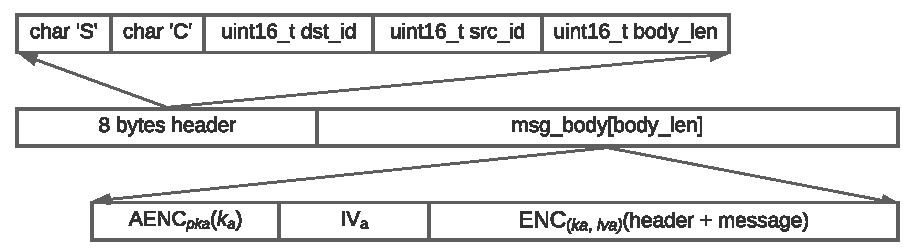
\includegraphics[width = .80\textwidth]{pic/msg-format.pdf}
  \caption{Targeted Transmission Message Forma}
  \label{fig:msg}
  \end{centering}
\end{figure}

\subsection{Broadcast Transmission}

When the SED$_a$ does a broadcast, it first generates an AES key $k_a$ and IV $iv_a$. 
Then, it uses AES-GCM to encrypt and authenticate the SCEWL header ($\mathcal{H}$) and body ($\mathcal{B}$), which outputs the ciphertext ($\mathcal{C}$) and tag ($\mathcal{T}$), e.g. $\mathcal{C}, \mathcal{T}$ = ENC$_{k_a, iv_a}(\mathcal{H} || \mathcal{B})$.
Then, it encrypts $k_a$ with its private key $sk_a$, e.g. $\mathcal{E}$=AENC$_{sk_a}(k_a)$.
Then, it sends out $\mathcal{M}$ = $\mathcal{H} || \mathcal{E}||iv_a||\mathcal{T}||\mathcal{C}$.
A caveat here is to calculate body length before the AES operation.

Whenever SED$_b$ receives a message $\mathcal{M}$, it first checks the $\mathcal{H}$ to see if the message is a broadcast.
Then, it uses SED$_a$'s public key $pk_a$ to decrypt the received ciphertext AES key $k_a$, e.g. $k_a$ = ADEC$_{pk_a}($AENC$_{sk_a}(k_a))$.
Then, it uses $k_a, iv_a$ to decrypt and authenticate the message, e.g. $\mathcal{C'}, \mathcal{T'}$ = DEC$_{k_a, iv_a}(\mathcal{C})$.
It compares $\mathcal{T'}$ and $\mathcal{T}$.
If they do not match, discard.
Otherwise, $\mathcal{C'}$ = $\mathcal{H}||\mathcal{B}$.

\subsection{Key Generation and Storage}

Below are the details Key generation for asymmetric encryption:
\begin{itemize}
  % \item[Step1.]
  \item[Step 1.] When adding SED$_k$ ($k$ refers to \verb|SCEWL_ID|) to a deployment, SSS generates a pair of RSA keys ($pk_k$, $sk_k$) for SED$_k$.
  SSS stores the keys in files as $k.pub$, $k.pri$ at its local filesystem.
  
  We implement \textbf{keygen} (with \verb|SCEWL_ID| as a parameter) application to generate key pair ($pk_k$ and $sk_k$) for each provisioned SED$_k$ first, then invoke \textbf{create\_secrets.py} to output the \textbf{key.h} which will be used to compile the SED$_k$ controller.

  This step runs the script from \textbf{dockerfiles/2b\_create\_sed\_secrets.Dockerfile} file.

  \item[Step 2.] When building controller for SED$_k$, the key pair ($pk_k$, $sk_k$) will be copied from the sss container to this controller container.
  
  At the time of building the controller of SED's.
  We change \textbf{dockerfiles/2c\_build\_controller.Dockerfile} to copy \textbf{key.h} from the SSS container to the controller container.

  \item[Step 3.] At registration stage, the SED$_k$ uses its own private key $sk_k$ to sign the registration message (with padding to 512 bits) and send it to the SSS.
  It sends out $\mathcal{M}$ = $\mathcal{H} || $SIG$_{sk_k}(\mathcal{B}, \mathcal{H})$, $\mathcal{B}$ = $k$ $||$ $op$ ($op$ refers the register operation).
  If $k$ is in our provisoned SED list, SSS will use the associated public key $pk_k$ to verify this message, e.g. $\mathcal{H'}, \mathcal{B'}$ = VER$_{pk_k}$(SIG$_{sk_k}(\mathcal{H}, \mathcal{B})$).
  Upon a successful verification ($\mathcal{H}$ == $\mathcal{H'}$), SSS finish the registration for SED$_k$, adds $k$ to a dedicated list, and sends the public keys of all other provisoned SEDs to SED$_k$.
  
  We implement \textbf{auth} application to verify the signed message, modify the \textbf{sss.py} to verify the provioned SEDs and send out the public keys of other provisoned SEDs.

  \item[Step 4.] The deregistration stage is similar to registration.
  SED$_k$ will delete other public keys first, then uses its own private key $sk_k$ to sign the deregistration message and send it to the SSS.
  It sends out $\mathcal{M}$ = $\mathcal{H} || $SIG$_{sk_k}(\mathcal{B}, \mathcal{H})$, $\mathcal{B}$ = $k$ $||$ $op$ ($op$ refers the deregister operation).
  If $k$ is in our provisoned SED list and in our dedicated list, SSS will use the associated public key $pk_k$ to verify this message.
  Upon a successful verification, SSS will remove SED$_k$ from the dedicated list.

  \item[Remove SED.] When removing SED$_k$, SSS will remove the key pair ($pk_k$, $sk_k$).
\end{itemize}

  \subsection{Prevent Replay Attack}
  For communication between the SEDs, a sequence number of 4 bytes is added in front of the message body. Each SED maintains a pair of sequence number table in memory of other SEDs. Two sequence numbers represent bidirectional transmission between two SEDs. To prevent the replay attack, receiver SED needs to cross-check between the received value from the message and the value from the table.
 
Explanation:
  \begin{itemize}
  \item Suppose there are 5 ($a, b, c, d, e$) SEDs in the system.
  \item Each SED maintains a pair of sequence number table of other SEDs with the initial value of zero.
  \item  Example: At the beginning sequence table for SED $b$:

    \begin{center}
  \begin{tabular}{ |c|c|c| } 
   \hline
  \textbf{SED ID} & \textbf{SQ\_send} & \textbf{SQ\_receive}\\
 	\hline \hline
 	a & 0 & 0 \\ 
	c & 0 & 0 \\ 
 	d & 0 & 0 \\ 
 	e & 0 & 0 \\ 
	 \hline
\end{tabular}
\end{center}
Here each row represents a pair of sequence number.
Row $a$ here signifies the sequence number for communication between the SED pair $(a,b)$. $SQ\_send$ is number of communications from SED $b$  to SED $a$. $SQ\_receive$ denotes number of messages that $b$ received from $a$. SED $a$ will have the same values in opposite position.

  \item Suppose SED$_a$ communicates with the SED $b$. SED $a$ gets the 
   $SQ\_send$ value of SED$_b$ from its table, increments it by one, and then adds it in front of the message body. 
  \item After successful decryption of the message, SED$_b$ checks the received sequence number from the message and $SQ\_receive$ sequence number of SED$_a$ from it's table in memory.
  \item The received message is valid only if the message sequence number is greater than the sequence number from the table. For a valid message, the receiver SED $b$ copies the sequence from the message to it's table. So, the  $SQ\_send$ for $b$ in SED$_a$'s table will be the same as $SQ\_receive$ for $a$ in the SED$_b$'s table.
  \item After communication sequence table for SED $b$:
    \begin{center}
  \begin{tabular}{ |c|c|c| } 
   \hline
  \textbf{SED ID} & \textbf{SQ\_send} & \textbf{SQ\_receive}\\
 	\hline \hline
 	a & 0 & 1 \\ 
	c & 0 & 0 \\ 
 	d & 0 & 0 \\ 
 	e & 0 & 0 \\ 
	 \hline
\end{tabular}
\end{center}
\item Similarly, SED$_a$'s table after this communication:
    \begin{center}
  \begin{tabular}{ |c|c|c| } 
   \hline
  \textbf{SED ID} & \textbf{SQ\_send} & \textbf{SQ\_receive}\\
 	\hline \hline
 	b & 1 & 0 \\ 
	c & 0 & 0 \\ 
 	d & 0 & 0 \\ 
 	e & 0 & 0 \\ 
	 \hline
\end{tabular}
\end{center}
\item Similarly, suppose SED$_b$ twice sends messages to SED$_c$ and once receives the message from SED$_c$. Now the table for SED $b$ should be:
    \begin{center}
  \begin{tabular}{ |c|c|c| } 
   \hline
  \textbf{SED ID} & \textbf{SQ\_send} & \textbf{SQ\_receive}\\
 	\hline \hline
 	a & 0 & 1 \\ 
	c & 2 & 1 \\ 
 	d & 0 & 0 \\ 
 	e & 0 & 0 \\ 
	 \hline
\end{tabular}
\end{center}
    \end{itemize}


\subsection{Build Process}

  \begin{itemize}
    \item \textbf{dockerfiles/1a\_create\_sss.Dockerfile}
    \begin{enumerate}
      \item Copy \textbf{rsa} folder to sss container.
      \item Copy \textbf{create\_secret.py} folder to sss container.
      \item Copy \textbf{sss.py} folder to sss container.
      \item Create a file (\textbf{provisoned\_list}) to store the provisoned SEDs
    \end{enumerate}
    \item \textbf{dockerfiles/2b\_create\_sed\_secrets.Dockerfile}
    \begin{enumerate}
      \item Create a folder in sss container to store the provisioned SEDs secrets (key pairs).
      \item Write provisoned SCEWL\_ID to the \textbf{provisoned\_list}.
      \item \textbf{keygen} is invoked to generate the key pair.
      \item \textbf{create\_secret.py} is invoked to generate the \$\{SCEWL\_ID\}\_publickKey.
    \end{enumerate}
    \item \textbf{dockerfiles/2c\_build\_controller.Dockerfile}
    \begin{enumerate}
      \item Copy the \textbf{\$\{SCEWL\_ID\}\_publickKey} to controller container.
    \end{enumerate}
  \end{itemize}

\section{Implementation}
\subsection{Critical Functions and Files}
\begin{itemize}
  \item \textbf{aes-gcm crypto lib}: message encryption and decryption (controller).
  \item \textbf{rsa}
  \begin{enumerate}
    \item \textbf{keygen}: key pairs generation (sss).
    \item \textbf{auth}: registration message authentication (sss).
    \item \textbf{crypto lib}: aes\_key encryption and decryption, message signature and authentication (controller).
  \end{enumerate}
  \item \textbf{create\_secret.py}: key file generation and deletion.
  \item \textbf{provisoned\_list}: store the provisoned SCEWL ids.
  \item \textbf{sss.py}: check the provisoned SEDs.
  \item \textbf{controller.c}: add message encryption, decryption, and authentication, update keys.
  \item \textbf{controller.h}: critical structures and macros.
  \item others key files.
\end{itemize}


% \section{Flag Protection}

% \subsection{\textsf{D}}


\end{document}
%==============================================================================
